\documentclass[a4paper,10pt]{scrartcl}

\usepackage[utf8]{inputenc}
\usepackage[ngerman]{babel}
\usepackage[T1]{fontenc}
\usepackage{amsmath}
\usepackage[section]{placeins}
\usepackage{graphicx}
\usepackage{esvect}


\title{Praktikum B Vorbereitung zu Versuch "wk"}
\author{Leon Machtl und Raphael Lehner}
\date{23.01.2020}

\begin{document}
	\maketitle
	\tableofcontents
	\newpage
	
	
	
	


	
	\section{Einleitung zum Versuch}
		Beim Windkanal handelt es sich um eine kontrollierbare Testumgebung für das aerodynamische Verhalten eines einer Strömung ausgesetzten Objekts. Dabei findet er heutzutage Anwendung in der Fahrzeugindustrie, sowie der Luft- und Raumfahrttechnik. Auch in der Architektur finden sich Anwendungen des Windkanals. Zudem wird er bei Sportarten, wie zum Beispiel Skispringen genutzt, um die geeignetste Körperhaltung zu finden. Die experimentelle Durchführung und Strömungsvisualisierung ist immer noch relevant, obwohl man durchaus die aerodynamischen Eigenschaften auch sehr gut am Computer simulieren kann.
		In diesem Praktikumsversuch werden die Grundlagen der Strömungslehre und der grundlegenden Parameter des vorhandenen Windkanals genauer untersucht. So wird unter anderem ein Strömungsprofil an der
		Messstrecke mit einem Anemometer aufgenommen und anschließend durch eine dreidimensionale Auftragung visualisiert. Außerdem soll eine Eichkurve für die Strömungsgeschwindigkeit zur am Gebläse angelegten Spannung aufgenommen werden. Anschließend werden mit dem Versuchsaufbau die Widerstandsbeiwerte (\(c_{w}\)-Werte) verschiedener vorgegebener Objekte bestimmt, um dann die experimentellen Beiwerte mit bekannten Tabellenwerten zu vergleichen. Im letzten Versuchsteil geht es um die Tragflächenphysik. Dabei soll im Rahmen des Praktikums das aerodynamische Verhalten verschiedener Tragflächenmodelle untersucht werden.
		
		\subsection{Windkanal nach Eiffel}
		
		Hierbei handelt es sich um die einfachste Form eines Windkanals (offene Bauart). Bei dieser Art Kanal wird Umgebungsluft über eine Öffnung angesaugt.
		Dort befinden sich üblicherweise mehrere Siebe und Gleichrichterelemente, die die eventuell verwirbelte Außenluft gleichrichten sollen.
		Die Luft gelangt dann in die Düse mit einer Querschnittsverengung und somit einer Geschwindigkeitserhöhung. In der darauffolgenden Messstrecke und dem Diffusor wird der Querschnitt wieder vergrößert, was wieder zu einer verlangsamung und einer Druckerhöhung führt, wodurch die Effizienz des hier verbauten Rotors erhöht wird. Nach dem Rotor wird die Luft wieder an die Umgebung
		abgegeben. Die saugende Anordnung des Gebläses am Ende des Kanals hat den Vorteil, dass so die
		Rotorwirbel nicht in den Messbereich gelangen. Die
		offene Bauart besitzt jedoch auch einige Nachteile. So muss die Messstrecke im Betrieb des Kanals
		immer von der Umgebung abgedichtet sein, da ansonsten im Messbereich die Luft seitlich
		eingesaugt wird und somit die vorgeschaltete Düse mit Gleichrichter ihre Wirkung verliert. Dadurch wird das experimentieren sehr erschwert, da die verwendete Messtechnik zum einen nicht in
		die Strömung geraten soll, andererseits aber auch nicht zu Undichtigkeiten in dem Bereich führen darf,
		wenn sie außerhalb liegt. Außerdem hat ein solcher Windkanal einen relativ schlechten Gütegrad, welcher
		sich aus dem Verhältnis der Strahlleistung zur Gebläseleistung ergibt. Die Ursache dafür ist, dass die Strömung aus der ruhenden Außenluft heraus zuerst beschleunigt werden muss und nach
		Durchlaufen des Kanals wieder auf ruhende Luftmassen trifft, wodurch sie wieder gebremst wird.
		
		\subsection{Windkanal Göttinger Bauart}
		
		Die geschlossene Bauart eines Windkanals soll die Nachteile der offenen Bauart umgehen. Daher wird hier die nach dem Gebläse ausgestoßene Luftmasse über einen Kanal wieder zur Düse
		zurückgeführt und erneut eingesaugt, so dass der Kreislauf eines geschlossenen Strömungssystems entsteht. Auch wenn die Versuchsstrecke teilweise zur Umwelt hin geöffnet ist, bleibt die Strömung größtenteils laminar, da die strömende Luft immer wieder durch die Gleichrichter fließt. 
		Dabei muss das Gebläse möglichst weit von der Düse entfernt sein, da ansonsten starke Verwirbelungen entstehen können, die unter Umständen in den Messbereich geraten. Das stellt einen Nachtteil im Vergleich zur offenen Bauart dar. Eine
		Möglichkeit, diesen zu umgehen, sind in den Kurvensegmenten angebrachte Leitschaufeln, die die Wirbel ”zerschneiden” und somit auflösen.
		Zudem leiten sie die Luft um die Kurve und vermindern dadurch Turbulenzen, die durch die Richtungsänderung der Strömung entstehen könnten. Eine weitere Möglichkeit
		stellt die Vergrößerung des Kanalquerschnitts dar, was eine Verlangsamung und stärkeren Druck zur Folge hätte. Die beste Art dies zu tun, ist die
		Aufweitung nach dem Gebläse fließend bis hin zur Düse fortzusetzen, wo sie ihr Maximum erreicht.
		Einfacher ist es die Querschnittsvergrößerung durch eine sogenannte Vorkammer erst kurz vor der
		Düse bei den Gleichrichterelementen vorzunehmen. Diese Methode ist allerdings nicht ganz so gut, wie die langsame Vergrößerung.
		
		\subsection{Geschwindigkeitsmessung}
		
		Mit folgenden Geräten kann man die Strömungsgeschwindigkeit eines Fluids messen.
		\begin{itemize}
			\item Flügelradanemometer
			\begin{itemize}
				\item besitzt einen kleinen Rotor
				\item von der Luftströmung
				angetrieben
				\item Reibungswiderstand verursacht die Lagerung
				des Flügelrades
				\item Ermittlung der Strömungsgeschwindigkeit über Winkelgeschwindigkeit des Rotors
				\item auch bei niedrigen Geschwindigkeiten nutzbar
				\item keine punktuellen Messungen möglich
				\item Gerät ist relativ hoher Störfaktor
			\end{itemize}
			\item Prandtl'sches Staurohr
			\begin{itemize}
				\item bekanntestes Staudruckanemometer
				\item Verwendung vor allem in Luftfahrt
				\item Geschwindigkeitsmessung relativ zur Umgebungsluft
				\item messung Differenz Gesamtdruck und statischem Druck
			\end{itemize}
		\end{itemize}
	
		\subsection{Tragflächenprofile}
			\begin{itemize}
				\item Klassisches Profil
				\begin{itemize}
					\item auch bei niedriger Geschwindigkeit viel Auftrieb
					\item hoher Strömungswiderstand
					\item Umschlagpunkt weit vorne
					\item Strömungsabriss erst bei steilen Anstellwinkeln
				\end{itemize}
				\item Symmetrisches Profil
				\begin{itemize}
					\item Wassertropfenform
					\item Bei 0 Grad Anstellwinkel kein Auf- oder Abtrieb
					\item Gleiche Eigenschaften bei positiven und negativen Winkeln
					\item Anwendung bei Kunstflugzeugen
					\item Im Versuch: 17\% Profildicke, 37,5\% Dickenrücklage
				\end{itemize}
				\item Laminares Profil
				\begin{itemize}
					\item geringe Profildicken
					\item weite Dickenrücklage
					\item Unterseite S-förmig
					\item Umschlagpunkt möglichste weit hinten, damit laminare Strömung niedrigen Luftwiderstand verursacht
					\item erfordern höhere Strömungsgeschwindigkeit für Auftrieb 
					\item glatte Oberfläche
					\item relativ abrupter Strömungsabriss schon bei kleinen Anstellwinkeln
					\item Anwendung bei Passagierflugzeugen
					\item Im Versuch: Dicke 10\%, Dickenrücklage 42\%
				\end{itemize}
			\end{itemize}
		
			\subsection{Charakteristsiche Punkte an Flügelprofil}
				\begin{itemize}
					\item Staupunkt
					\begin{itemize}
						\item Punkt, an dem Luftströmung genau senkrecht auf die Profiloberfläche
						auftrifft
						\item Strömung komplett abgebremst
						\item Druckaufbau
						\item gleichmäßige Aufteilung auf Ober- und Unterseite
						\item zunächst Ausbildung laminarer Grenzschicht
					\end{itemize}
					\item Umschlagpunkt
					\begin{itemize}
						\item bei kleinen Winkeln: Fortsetzung laminare Strömung solange beschleunigt
						\item Auf Oberseite: Bis größte Dicke
						\item Umschlag von laminar nach turbulent
						\item Teilchen bewegen sich auch quer zu Anströmrichtung, aber nach Kontinuitätssatz muss Hauptstrom erhalten bleiben und somit erhöhte Geschwindigkeit der Teilchen
						\item Aufgrund der dafür nötigen Energie, nimmt Widerstand zu 
						\item Auf Unterseite: laminare Grenzschicht wird weiter hinten durch Rauheit der Profilfläche zerstört 
					\end{itemize}
					\item Ablösungspunkt
					\begin{itemize}
						\item Luftströmung kann Profiloberfläche besser folgen, je schneller sie ist
						\item turbulente Strömung folgt besser als laminare
						\item Profilhinterkante: Abnahme Geschwindigkeit durch Druckanstieg
						\item Strömung kann sich nicht mehr an Profiloberfläche halten, es folgt Strömungsabriss
						\item Ab da nur noch Widerstand, kein Auftrieb mehr
					\end{itemize}
				\end{itemize}
				
				Die drei Punkte sind nicht stationär, sondern ändern sich bei verschiedenen Anstellwinkeln. Erreicht Ablösungspunkt Profilnase, hat dies einen vollständigen Strömungsabriss zur Folge und der Auftrieb bricht zusammen.
		
	\section{Fragen zur Vorbereitung}
		\subsection{Frage 1}
			Leiten Sie die Kontinuitätsgleichung mit laminarer Strömung durch eine geschlossene Röhre
			her!\\
			\\
			Aufgrund der Massenerhaltung muss die Masse, die in die Röhre fließt gleich der Masse sein, die aus der Röhre wieder hinaus fließt. Die Gesamtmasse ändert sich also nicht.
			\begin{align*}
			\dot m=0
			\end{align*}
			Somit gilt für den eintretenden Massestrom \(\dot m_{1}\) und den ausstretenden Massestrom \(\dot m_{2}\)
			\begin{align}
			\dot m_{1}=\dot m_{2}
			\end{align}
			Die zeitliche Änderung der Masse wird beschrieben durch 
			\begin{align*}
			\dot m=\rho \dot V
			\end{align*}
			Wobei \(V\) das Volumen bezeichnet. Die zeitliche Änderung des Volumens, also der Volumenstrom ergibt sich seinerseits durch
			\begin{align*}
			\dot V=vA
			\end{align*}
			wobei \(v\) die mittlere Strömungsgeschwindigkeit und \(A\) die betreffende Querschnittsfläche bezeichnet. Somit folgt aus (1):
			\begin{align*}
			\rho_{1}v_{1}A_{1}=\rho_{2}v_{2}A_{2}
			\end{align*}
			und für ein inkompressibles Fluid mit \(\rho_{1}=\rho_{2}\)
			\begin{align*}
			v_{1}A_{1}=v_{2}A_{2}
			\end{align*}
			
		\subsection{Frage 2}
			Skizzieren Sie die Unterschiede zwischen einer laminaren und einer turbulenten Strömung.
			Wann ist eine Strömung stationär?\\
			\\
			Laminare Strömung:
			\begin{itemize}
				\item Bewegung von Flüssigkeiten und Gasen
				\item Fluid strömt in sich nicht vermischenden Schichten
				\item bei Übergangsgebiet senkrecht zur Strömungsrichtung keine sichtbaren Turbulenzen zwischen unterschiedlichen Strömungsgeschwindigkeiten
				\item Reynoldszahl kleiner als kritischer Wert \(Re_{krit}\)
				\item Bahn eines Teilchens wird durch \glqq Stromfaden\grqq{} beschrieben
			\end{itemize}
			
			Turbulente Strömung:
			\begin{itemize}
				\item Bewegung von Fluiden (Flüssigkeiten, Gase)
				\item Verwirbelungen treten auf
				\item Teilchen werden kontinuierlich durcheinander gemischt
				\item Bahn eines Teilchens kann nicht vorhergesagt werden
				\item Reynoldszahl größer als der kritische Wert \(Re_{krit}\)
				\item in Rohr entsteht Verwirbelung durch den Geschwindigkeitsunterschied der Strömung in der Rohrmitte gegenüber der Strömung nahe der Wand des Rohrs
			\end{itemize}
			
			Eine Strömung ist stationär, wenn sich sowohl die Strömungsgeschwindigkeit, als auch die Querschnittsfläche der Strömung nicht zeitlich ändern, also an jedem einzelnen Ort gilt:
			\begin{align*}
			\dot v=\dot A=0
			\end{align*}
			Allerdings können sich \(v\) und \(A\) zwischen verschiedenen Orten sehr wohl variieren, die Ableitung nach dem Ort muss also nicht zwingend 0 sein. In einer stationären Strömung entsprechen die Stromlinien auch den Bahnlinien und die Teilchen bewegen sich auf den zeitlich unveränderten Stromlinien.
			
		\subsection{Frage 3}
			Eine wichtige Beschreibung strömender Fluide liefert die Bernoulli-Gleichung. Leiten Sie diese
			für reibungsfreie, inkompressible Fluide anhand der Abbildung wk.2 aus dem Praktikumsskript her. Gehen Sie hierbei von der Energieerhaltung idealer, reibungsfreier Fluide aus.\\
			\\
			Die Arbeit ist gegeben durch Änderung der Energie, also hier:
			\begin{align*}
			W=\Delta E_{Druck}+\Delta E_{kin}
			\end{align*}
			\begin{align*}
			W=F\Delta x + \Delta E_{kin}
			\end{align*}
			Mit der durch den Druck verübten Kraft \(F=pA\) ergibt sich
			\begin{align*}
			W=pA\Delta x=p\Delta V +\Delta E_{kin}
			\end{align*}
			wobei \(p\) den Druckunterschied zwischen den beiden beiden betrachteten Stellen bezeichnet. Damit erhält man
			\begin{align*}
			W=(p_{2}-p_{1})\Delta V +\Delta E_{kin}
			\end{align*}
			Die Änderung der kinetischen Energie ergibt sich wie folgt:
			\begin{align*}
			\Delta E_{kin}=\frac{1}{2}\Delta m(v_{2}^{2}-v_{1}^{2})
			\end{align*}
			mit \(\Delta m=\rho \Delta V\) folgt dann, wenn man auf beiden Seiten durch \(\Delta V\) dividiert und verwendet, dass die Gesamtenergie im System konstant bleiben muss:
			\begin{align*}
			(p_{2}-p_{1})+\frac{1}{2}\rho (v_{2}^{2}-v_{1}^{2})=const.
			\end{align*}
			\begin{align*}
			p_{1}+\frac{1}{2}\rho v_{1}^{2}=p_{2}+\frac{1}{2}\rho v_{2}^{2}
			\end{align*}
			somit folgt
			\begin{align*}
			p+\frac{1}{2}\rho v^{2}=p_{0}=const.
			\end{align*}
			wobei \(p=p_{stat}\) und \(\frac{1}{2}\rho v^{2}\) den Staudruck bezeichnet.
			
		\subsection{Frage 4}
			Berechnen sie den relativen Druckabfall strömender Luft (\(\rho=1,293\frac{kg}{m^{3}}\), \(p_{0}=1bar\)) bei
			einer Strömungsgeschwindigkeit von 250 km/h.\\
			\\
			Der relative Druckabfall ergibt sich durch das Verhältnis der Druckänderung zum Ausgangsdruck. Er errechnet sich also wie folgt:
			\begin{align*}
			\frac{p_{1}-p_{2}}{p_{1}}
			\end{align*}
			Beim Ausgangsdruck ist die Luft in Ruhe, aus der Bernoulli-Gleichung folgt also
			\begin{align*}
			\rho_{1}=p_{0}=1bar=100000Pa
			\end{align*}
			Für \(p_{2}\) gilt dann
			\begin{align*}
			p_{2}=p_{0}-\frac{1}{2}\rho v^{2}=100000Pa-\frac{1}{2}\cdot 1,293\frac{kg}{m^{3}}\cdot (\frac{250}{3,6}\frac{m}{s})^{2}=9,7\cdot 10^{4}Pa
			\end{align*}
			Und somit ergibt sich für den relativen Druckabfall:
			\begin{align*}
			\frac{p_{1}-p_{2}}{p_{1}}=\frac{100000Pa-(100000Pa-\frac{1}{2}\cdot 1,293\frac{kg}{m^{3}}\cdot (\frac{250}{3,6}\frac{m}{s})^{2})}{100000Pa}=0,03=3\%
			\end{align*}
			
		\subsection{Frage 5}
			Welche Bedeutung hat der \(c_{w}\)-Wert in der Aerodynamik? Wie wird er im Versuch experimentell
			bestimmt?\\
			\\
			Der \(c_{w}\)-Wert ist ein Maß für den Strömungswiderstand eines Körpers, der von einem Fluid umströmt wird. Er besitzt keine Dimension. Er wird auch als Strömungswiderstandskoeffizient bezeichnet. Seine Bedeutung für die Aerodynamik wird deutlich, wenn man sich anschaut, wie er definiert ist:
			\begin{align*}
			c_{w}=\frac{2F_{w}}{\rho v^{2}A}
			\end{align*}
			Wobei \(F_{w}\) die Widerstandskraft, \(A\) die betrachtete Fläche und der Rest die Staudichte bezeichnen. Man sieht also, dass der \(c_{w}\)-Wert dazu dient, die Kraft, welche durch eine Strömung, die auf eine Fläche trifft, ausgeübt wird, zu bestimmen. In der Aerodynamik versucht man daher z.B. beim Bau von Autos diese so zu designen, dass sie einen möglichst geringen \(c_{w}\)-Wert besitzen, um die Widerstandskraft klein zu halten, damit das Auto nicht zu stark gebremst wird.\\
			Der \(c_{w}\)-Wert kann experimentell im Windkanal bestimmt werden, indem man denzu betrachtenden Körper auf Kraftsensoren platziert und die Widerstandskraft damit misst. Dann kann man mit den bekannten Dichte- und Geschwindigkeitswerten, sowie der Stirnfläche des Körpers, bzw. bei Flügeln der Flügelfläche (Auftriebsfläche) den jeweiligen \(c_{w}\)-Wert berechnen. Bei sehr komplexen Gegenstandsformen kann dies äußerst kompliziert werden, so dass man unter Umständen auf eine numerische Berechnung zurückgreift. Im heutigen Versuch handelt es sich bei den Kraftsensoren um eine Umlenkvorrichtung.
			
		\subsection{Frage 6}
			Was ist der Magnuseffekt? Nennen Sie ein alltägliches Beispiel!\\
			\\
			Durch den Magnus-Effekt wird die Wirkung einer Querkraft beschrieben, die ein rotierender Körper in einer Strömung erfährt. Diese Querkraft wirkt senkrecht zur Anströmrichtung, sowie senkrecht zur Rotationsachse des rotierenden Körpers. Für die Erklärung dieses Effektes betrachten wir eine rechtsdrehende Kugel, welche sich in einer von links nach rechts verlaufenden Strömung befindet. Durch diese Drehbewegung werden die Teilchen, welche sich auf der oberen Seite der Kugel befinden, beschleunigt, wohingegen die auf der unteren Seite durch die Bewegung Verlangsamt werden. Somit ist die Geschwindigkeitsverteilung nicht mehr homogen. Damit folgt dann direkt aus der Bernouilli Gleichung, dass auch die Druckverteilung nicht mehr homogen sein kann. Die wirkende Querkraft ergibt sich dann durch die Beziehung:
			\begin{align*}
			F=\Delta p A
			\end{align*}
			wobei \(\Delta p\) den Druckunterschied zwischen der Ober- und Unterseite der rotierenden Kugel bezeichnet und \(A\) die Querschnittsfläche der Kugel. Im Alltag kann man den Magnuseffekt zum Beispiel im Sport betrachten. So wird er im Fußball genutzt, um dafür zu sorgen, dass der Ball in der Luft seine Richtung ändert, oder auch beim Tischtennis oder Tennis in ähnlicher weise (Topspin, Slice).
			\FloatBarrier
			\begin{figure}[h]
\centering
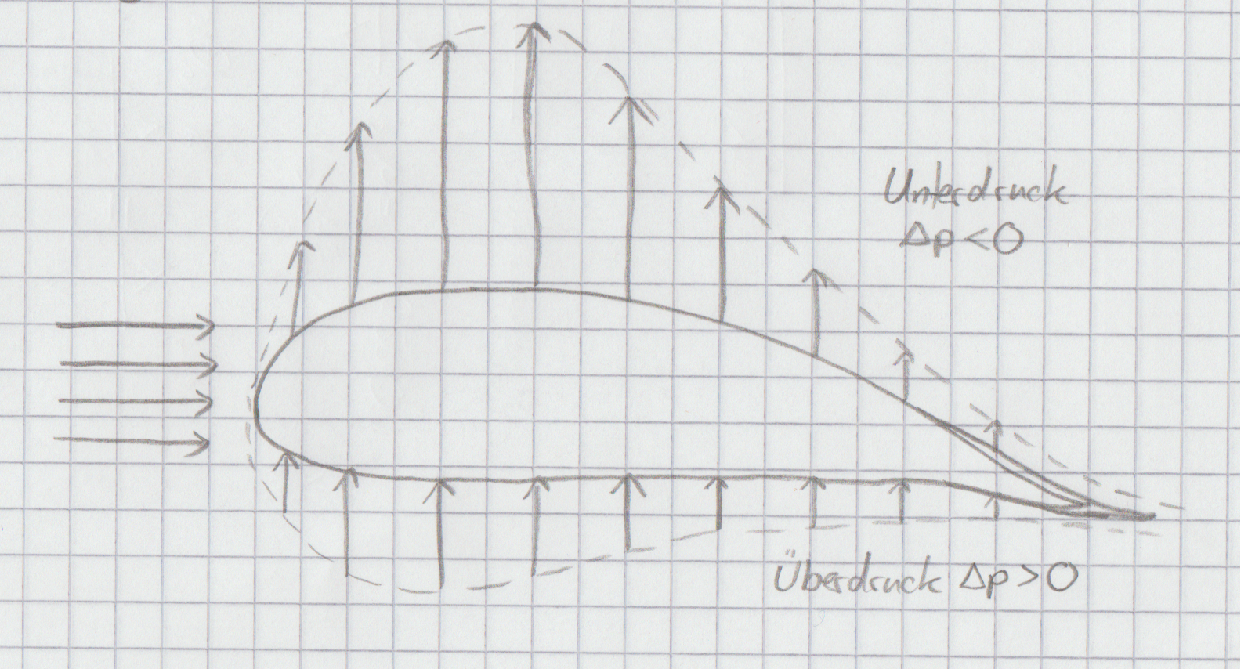
\includegraphics[width=0.7\textwidth]{./Bilder/wk2}

\end{figure}
\FloatBarrier
			
		\subsection{Frage 7}
			In (Abb. wk.10 im Skript) ist ein Tragflächenprofil skizziert. Beschreiben Sie qualitativ die Entstehungsgrundlage
			der Auftriebskraft \(F_{A}\).\\
			\\
			In der Zeichnung wird ein Laminares Profil dargestellt. Dies hat zur Folge, dass der Umschlagpunkt aufgrund der S-förmigen Unterseite sehr weit hinten liegt und daher auf der Unterseite weitestgehend eine laminare Strömung herrscht, die eng an der Profiloberfläche verläuft. Auf der Oberseite folgt die Strömung nicht solange der Profilfläche, weshalb auf der Oberseite rasch eine schnelle, turbulente Strömung entsteht. Durch die erhöhte Geschwindigkeit ist der Druck auf der Oberseite nun höher, als auf der Unterseite mit der laminaren, langsameren Strömung. Es entsteht also auf der Oberseite des Profils ein Unterdruck und auf der Unterseite ein Überdruck, wodurch die Tragfläche einen Auftrieb nach oben erfährt.
			\FloatBarrier
\begin{figure}[h]		
		\centering
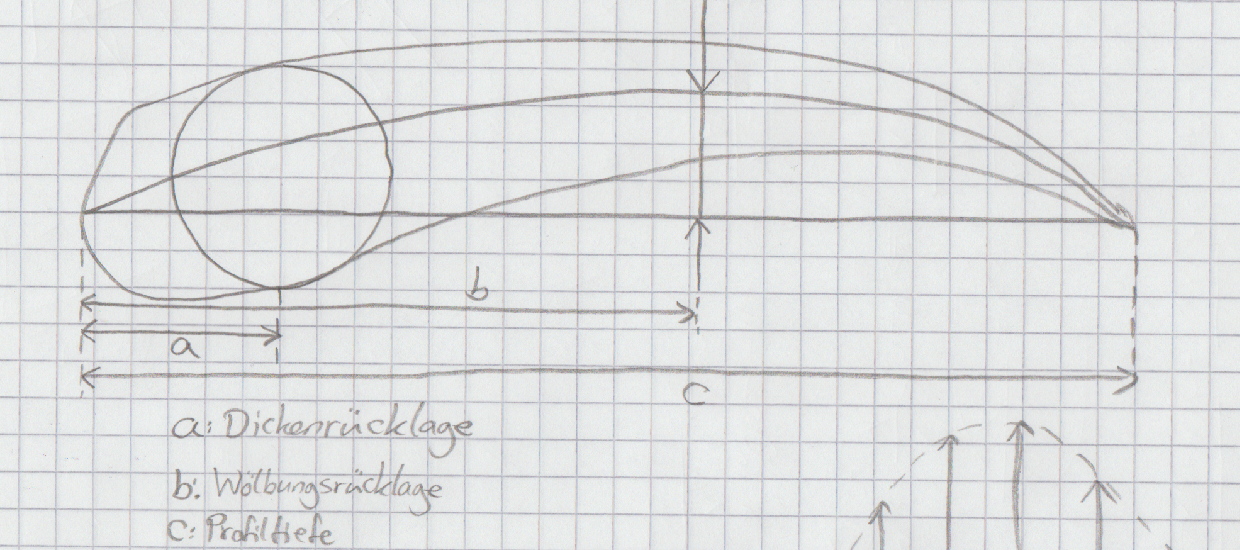
\includegraphics[width=0.7\textwidth]{./Bilder/wk1}

\end{figure}
\FloatBarrier
	\end{document}